\section{Einleitung}

Im Rahmen des Klimarisiko-Stresstests 2022 konzentrierte sich die Bewertung physischer Risiken auf zwei extreme Wetterereignisse, die zentrale Klimarisiken in Europa darstellen: (1) eine große Überschwemmung und (2) eine schwere Dürre mit Hitzewelle \parencite{ECB2022ClimateStressTest}. Flussüberschwemmungen waren historisch betrachtet eine bedeutende Quelle physischer Risiken in Europa und werden aufgrund prognostizierter Niederschlagszunahmen voraussichtlich an Relevanz gewinnen.
Diese Arbeit fokussiert sich spezifisch auf das Flusshochwasserrisiko in Bayern, Deutschland. Diese Eingrenzung ermöglicht eine detaillierte Analyse der regionalen Auswirkungen und Anpassungsstrategien im Kontext physischer Klimarisiken für den bayerischen Immobiliensektor.

Im Folgenden wird beispielhaft gezeigt, wie Zitate, Bilder, Tabellen oder Quellcode in die Arbeit eingefügt werden können.

Extreme weather events, such as floods, heat waves, cold waves, droughts, and hurricanes, can generate a significant impact on a bank’s residential mortgage portfolio. Their impacts can be summarized as follows:
Damage to property as collateral: They can cause damage to homes and other properties, making it difficult for homeowners to make their mortgage payments to the bank.
Higher default rate: The bank will encounter higher default rates on mortgage loans in the region concerned. For instance, borrowers may become homeless because of severe damage to their properties and their wealth. Some borrowers may lose their jobs and find it hard to repay loans to the bank.
Lower property valuation: In addition to direct damage to a property, extreme weather events can lower the market valuation of properties in the region concerned. Other banks may cut their residential mortgage lending for the region. Insurance companies may increase insurance premiums on properties in the region. All these factors lead to lower property values in the region. Then, the bank will encounter higher loan-to-value (LTV) ratios on mortgage loans, higher credit risk estimates on mortgage loans, and higher capital required to support the mortgage lending business.
To deal with climate risks to banks, some bank regulators have taken steps to mitigate the risk of extreme weather events on residential mortgage loans. For example, the bank regulators of the EU, the USA, Canada, Australia, and Hong Kong have guidelines established for lenders to follow when evaluating the risk of default on a loan. These guidelines include requirements for lenders to assess the potential impacts of extreme weather events on a borrower’s ability to make payments. The Prudential Banking Authority of the UK encourages banks to consider insurance coverage on residential mortgages against climate catastrophes. This aims to ensure that lenders are adequately protected in an extreme weather event. Both the US and Australian regulators have developed guidelines for lenders to follow when providing relief to borrowers affected by extreme weather events. These guidelines include requirements for lenders to provide temporary payment relief and additional support for borrowers unable to make mortgage payments due to extreme weather. The Basel Committee makes it clear that banks should consider the possible impacts of extreme weather events on property values associated with collateralized loans and expects bank regulators to develop prudent valuation criteria for their jurisdictions [1].
The impact of extreme weather events on property values is a complex issue that has been the subject of much research in recent years. For instance, the types of climate hazard risks, the resilience of urban development, geolocation, types of buildings, types of economic activities in a region, etc., can affect how a climate hazard damages property values [2]. Banks have an urgent need to improve their property valuation models with multi-criteria techniques [3].
One challenge for bank regulators in managing climate risk on residential mortgage loans in a banking system is the lack of data and information about the potential impacts of extreme weather events. This makes it difficult for regulators to assess the risk of default on a loan and to develop effective strategies to mitigate this risk. In addition, there is a lack of understanding of the potential impacts of extreme weather events on the housing market. This can make it difficult for regulators to evaluate the potential impacts of climate change on the availability of housing and the cost of residential mortgages. Furthermore, there is a lack of agreement among regulators about how to best manage climate risks in the financial system. This can lead to a lack of coordination between regulators, making it difficult to effectively manage climate risk on mortgage loans.
This paper aims to propose a framework to integrate two extreme weather risk measures, namely, stressed PD (probability of default) and stressed LGD (loss given default), into existing credit risk management frameworks used by banks following the internal-rating-based (IRB) approach of Basel II [4]. Since the implementation of Basel II, before 2010, many banks have developed their own IRB systems built for credit risk assessment and capital requirement calculations. These IRB systems continue to be used under Basel III, effective in January 2020. According to Basel Committee rules, the IRB systems produce three major credit risk measures, namely, probability of default (PD), loss given default (LGD), and exposure at default (EAD). Bank regulators convert these three credit risk measures into the capital required for credit risk business. By integrating the proposed extreme weather risk measures, banks can easily conduct climate stress tests on their residential mortgage loans. Meanwhile, bank regulators can easily compare the climate risks of residential mortgage loans from different banks.
Traditional stress tests used by banks aim to evaluate worst-case losses resulting from undesirable economic scenarios. The stress scenarios can be specified by related regulators every year or on an ad hoc basis, associated with a bank’s historical experience, based on expert projections, and/or grounded in some statistical confidence levels of market or economic outcomes. Some banks prefer to consider a consistent set of stress scenarios. This enables them to compare the stressed losses of their different business units and perform a trend analysis of stressed losses. The stressed loss results under consistently applied scenarios can be conveniently translated into internal capital allocation and credit pricing. Such methodologies of economic stress tests can be converted to climate stress tests. The goal of the climate stress test is to set an extreme weather scenario and evaluate related losses. Extreme weather events did not happen very often in the past, but they will be more frequent in the future. Bank regulators may occasionally give banks some climate stress scenarios to consider. However, the banks themselves do have an urgent need to routinely evaluate stressed losses due to extreme weather events and determine their business and lending strategies. This is because extreme climate events may arrive with short notice.
This paper considers a hypothetical case in which a bank wants to develop a routine climate stress test exercise for its portfolio of residential mortgage loans. The bank is determined to update the climate stress test results every 6 months, while most bank regulators perform the test at least once a year. This climate stress test exercise is complementary to the ad hoc climate stress tests required by the bank’s regulator. It is assumed that the bank routinely updates the PD and LGD of every residential mortgage loan and its related stressed loss arising from a predetermined and hypothetical extreme weather event. With simulation techniques and the assumptions of default correlation, this paper evaluates the stressed loss of the bank’s portfolio of residential mortgage loans. The results show that the bank can suffer a portfolio loss of 24.1% at the 99th percentile and of 39.04% at the 99.9th percentile. Such high portfolio losses come from the correlation between defaults and property damage caused by an extreme weather event. The results alert banks when planning their mortgage portfolios in terms of geolocational diversification, insurance against climate catastrophes, mortgage securitization, etc.
This paper will proceed as follows. Section 2 provides a literature review on the impacts of extreme weather on residential mortgage loans, credit risks in extreme weather conditions, and recent actions of bank regulators on climate risk management. Section 3 describes how the hypothetical case study is used in this paper. Section 4 discusses stress test assumptions and results. Section 5 concludes the paper.
\subsection{Zitate}
Menschen, die mit ihrem IQ prahlen, sind Versager.

\subsection{Bilder}
\begin{figure}[H] 
    \centering
    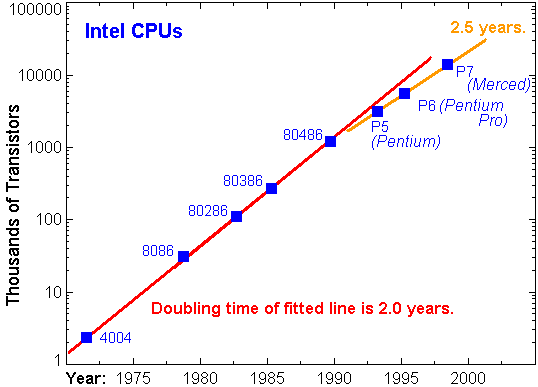
\includegraphics[width=0.5\textwidth]{figures/figure_example.png}
    \caption{Mooresches Gesetz}
\end{figure}

\subsection{Tabellen}
\begin{table}[H]
    \centering
    \begin{tabular}[H]{l|l|l}
        Bezeichnung & Kerne & TDP \\
        \hline
        Intel Core i5 & 6 & 111 W \\
        \hline
        AMD Ryzen 7 & 8 & 178 W \\
    \end{tabular}
    \caption{Prozessoren}
\end{table}


\subsection{Quellcode}
\begin{lstlisting}[language=java, caption=Hello World in Java, captionpos=b]
    class HelloWorld {
        public static void main(String[] args) {
            // Display the string.y
            System.out.println("Hello World!");
        }
    }
\end{lstlisting}
